\documentclass{beamer}
\usepackage[orientation=portrait,size=a0,scale=1.4,debug]{beamerposter}
\mode<presentation>{\usetheme{ZH}}
\usepackage{fontspec}
\usepackage{microtype}
\usepackage[english]{babel} % required for rendering German special characters
\usepackage{siunitx} %pretty measurement unit rendering
\usepackage{hyperref} %enable hyperlink for urls
\usepackage{ragged2e}
\usepackage[font=scriptsize,justification=justified]{caption}
\usepackage{array,booktabs,tabularx}
\usepackage{float}
\usepackage{subfig}

\newcommand{\sgn}{\operatorname{sgn}}
\newcommand{\conv}{\operatorname{conv}}
\newcommand{\vect}{\operatorname{vect}}
\DeclareMathOperator*{\argmin}{arg\,min}
\DeclareMathOperator*{\argmax}{arg\,max}
\newcommand*\diff{\mathop{}\!\mathrm{d}}
\newcommand{\Var}{\mathrm{Var}}
\newcommand*\ri{\mathop{}\!\mathrm{ri}}
\newcommand*\aff{\mathop{}\!\mathrm{aff}}
\newcommand*\dom{\mathop{}\!\mathrm{dom}}
\newcommand*\epi{\mathop{}\!\mathrm{epi}}
\newcommand*\diag{\mathop{}\!\mathrm{diag}}
\newcommand*\cov{\mathop{}\!\mathrm{cov}}
\newcommand*\var{\mathop{}\!\mathrm{var}}
\newcommand*\corr{\mathop{}\!\mathrm{corr}}

\newcolumntype{Z}{>{\centering\arraybackslash}X} % centered tabularx columns
\sisetup{per=frac,fraction=sfrac}

\title{Semi-parametric blind sources separation with \huge Kernel-ICA}
\author{Guillaume Ausset}
\institute[MASH]{Université Paris Dauphine}
\date{January 4, 2017}

% edit this depending on how tall your header is. We should make this scaling automatic :-/
\newlength{\columnheight}
\setlength{\columnheight}{107cm}

\begin{document}
\begin{frame}
\begin{columns}
	\begin{column}{.5\textwidth}
		\begin{beamercolorbox}[center]{postercolumn}
			\begin{minipage}{.98\textwidth}  % tweaks the width, makes a new \textwidth
				\parbox[t][\columnheight]{\textwidth}{ % must be some better way to set the the height, width and textwidth simultaneously
					\begin{myblock}{Introduction}
					It is rare for the quantity of interest and the quantity measured to perfectly match often our signal of interest $s \in \mathcal{R}^{m \times n}$ is actually mixed with itself. We will set up a certain number of recording devices, generally $n$ and from our recorded signals try to recover the sources. If we assume the sources are linearly mixed our problem is then:

						\begin{align*}
							x = A s
						\end{align*}

						where $x \in \mathcal{R}^{k \times n}$, $A \in \mathcal{R}^{k \times m}$. While not always true or needed we will assume that $A$ is square and invertible and call $A^{-1} = W$.

						We will see that the sole hypothesis of the independence of the $s_i$ is enough to find a solution to the problem.

						Because of the way the problem is posed one cannot hope to recover the real $s$ as for example a scaling or permutation of $A$ leaves the problem unchanged and we therefore cannot hope to recover the magnitudes (and therefore signs) of the $s_i$ or their order.
					\end{myblock}\vfill
					\begin{myblock}{ICA as an eigenvalue problem}
						We want to optimize a measure of independence of our estimated sources. Most approaches try to optimize an approximation of the mutual information. The measure chosen here \cite{Bach2002} is for two variables:
						\begin{align*}
							\rho_\mathcal{F} = \max_{f_1, f_2 \in \mathcal{F}} \corr (f_1(x_1), f_2 (x_2))
						\end{align*}
						By exploiting the kernel trick we can obtain
						\begin{align*}
							\rho_\mathcal{F} = \max_{f_1, f_2 \in \mathcal{F}} \corr ( \langle \Phi_1 (x_1), f_1 \rangle , \langle \Phi_2 (x_2), f_2 \rangle)
						\end{align*}
						We recognize a CCA problem and if we note $K_1$ and $K_2$ the respective Gram matrices (assuming they are centred) we get the problem:
						\begin{align*}
							\begin{pmatrix}
								0 & K_1 K_2 \\
								K_2 K_1 & 0
							\end{pmatrix} \begin{pmatrix}
								\alpha_1 \\ \alpha_2
							\end{pmatrix}
							= \rho \begin{pmatrix}
								K_1^2 & 0 \\
								0 & K_2^2
							\end{pmatrix} \begin{pmatrix}
								\alpha_1 \\ \alpha_2
							\end{pmatrix}
						\end{align*}
						This problem is unfortunately not well posed and will always be equal to $0$ for most kernels, we therefore adopt a regularized version as an estimator:
						\begin{align*}
							\rho_\mathcal{F} = \max_{f_1, f_2 \in \mathcal{F}} \frac{\cov (f_1(x_1), f_2 (x_2))}{(\var f_1 (x_1) + \kappa \lVert f_1 \rVert^2 _\mathcal{F} )^{1/2} (\var f_2 (x_2) + \kappa \lVert f_2 \rVert^2 _\mathcal{F} )^{1/2}}
						\end{align*}
						The problem estimated at the first order is then:
						\begin{align*}
							\begin{pmatrix}
								0 & K_1 K_2 \\
								K_2 K_1 & 0
							\end{pmatrix} \begin{pmatrix}
								\alpha_1 \\ \alpha_2
							\end{pmatrix}
							= \rho \begin{pmatrix}
								(K_1+\frac{N \kappa}{2} \mathbb{I})^2 & 0 \\
								0 & (K_2+\frac{N \kappa}{2} \mathbb{I})^2
							\end{pmatrix} \begin{pmatrix}
								\alpha_1 \\ \alpha_2
							\end{pmatrix}
						\end{align*}
						Of course we are interested in solving the $m$-variables problems, we can easily extend CCA to $m$ variables.
						%\begin{align*}
						%	&\begin{pmatrix}
						%		0 & K_1 K_2  & \cdots & K_1 K_m\\
						%		K_2 K_1 & 0 & \cdots & K_2 K_m \\
						%		\vdots & \vdots & \ddots & \vdots \\
						%		K_m K_1 & K_m K_2 & \cdots & 0
						%	\end{pmatrix} \begin{pmatrix}
						%		\alpha_1 \\ \alpha_2 \\ \vdots \\ \alpha_m
						%	\end{pmatrix} \\
						%	&= \rho \begin{pmatrix}
						%		(K_1+\frac{N \kappa}{2} \mathbb{I})^2 & 0  & \cdots & 0\\
						%		0 & (K_2+\frac{N \kappa}{2} \mathbb{I})^2 & \cdots & 0 \\
						%		\vdots & \vdots & \ddots & \vdots \\
						%		0 & 0 & \cdots & (K_m+\frac{N \kappa}{2} \mathbb{I})^2
						%	\end{pmatrix} \begin{pmatrix}
						%		\alpha_1 \\ \alpha_2 \\ \vdots \\ \alpha_m
						%	\end{pmatrix}
						%\end{align*}
						We can then transform that problem in the problem of finding the eigenvalues of:
						\begin{align*}
							&\tilde{\mathcal{K}}_\kappa = \begin{pmatrix}
								\mathbb{I} & r_\kappa (K_1)  r_\kappa (K_2)  & \cdots &  r_\kappa (K_1) r_\kappa (K_m)\\
								r_\kappa (K_2)  r_\kappa (K_1) & \mathbb{I} & \cdots & r_\kappa (K_2) r_\kappa (K_m) \\
								\vdots & \vdots & \ddots & \vdots \\
								r_\kappa (K_m)  r_\kappa (K_1) & r_\kappa (K_m) r_\kappa (K_2) & \cdots & \mathbb{I}
							\end{pmatrix} \\
							& r_\kappa (K_i) = K_i (K_i + \frac{N \kappa}{2} \mathbb{I})^{-1}
						\end{align*}
						We then optimize:
						\begin{align*}
							J(W) = -\frac{1}{2} \det \tilde{\mathcal{K}}_\kappa
						\end{align*}
					\end{myblock}\vfill
					\begin{myblock}{Reducing Complexity}
						If we decompose the $K_i$ as
						\begin{align*}
							K_i = G_i G_i^\intercal = U_i \Lambda_i U_i^\intercal
						\end{align*}
						with $\Lambda_i$ diagonal then if $R_i$ is $\Lambda_i$ regularized by $\lambda \to \frac{\lambda}{\lambda + N \kappa / 2}$ we have
						\begin{align*}
							\tilde{\mathcal{K}}_\kappa = (\mathcal{U} \mathcal{V}) \begin{pmatrix}
							\mathcal{R}_\kappa & 0 \\
							0 & \mathbb{I}
							\end{pmatrix} (\mathcal{U} \mathcal{V})^\intercal
						\end{align*}
						with
						\begin{align*}
							\mathcal{R}_\kappa =  \begin{pmatrix}
								\mathbb{I} & R_1 U_1^\intercal U_2 R_2  & \cdots &  R_1 U_1^\intercal U_m R_m \\
								 R_2 U_2^\intercal U_1 R_1 & \mathbb{I} & \cdots & R_2 U_2^\intercal U_m R_m \\
								\vdots & \vdots & \ddots & \vdots \\
								R_m U_m^\intercal U_1 R_1 & R_m U_m^\intercal U_2 R_2 & \cdots & \mathbb{I} \\
							\end{pmatrix}
						\end{align*}
						And therefore
						\begin{align*}
							\det \tilde{\mathcal{K}}_\kappa = \det \mathcal{R}_\kappa
						\end{align*}
						We will therefore make heavy use of incomplete Choleski decomposition to reduce the computational complexity.
					\end{myblock}\vfill
		}\end{minipage}\end{beamercolorbox}
	\end{column}
	\begin{column}{.5\textwidth}
		\begin{beamercolorbox}[center]{postercolumn}
			\begin{minipage}{.98\textwidth} % tweaks the width, makes a new \textwidth
				\parbox[t][\columnheight]{\textwidth}{ % must be some better way to set the the height, width and textwidth simultaneously
					\begin{myblock}{Optimization on the Stiefel Manifold}
						Our problem is
						\begin{align*}
							&\min_W J(W) \\
							\text{s.t } &W W^\intercal = \mathbb{I}
						\end{align*}
						The set $\{ W \mid W W^\intercal = \mathbb{I} \}$ has a particular geometry: it is Riemannian manifolds and most common optimization procedures can be performed on it \cite{Edelman1998}.
						The simplest implementation is steepest descent along geodesics in the direction of the gradient using the following: if $W, H \in \mathcal{R}^{m \times n}$ s.t $W^\intercal W = \mathbb{I}$ and $A = W^\intercal H$ skew-symmetric then the geodesic on the Stiefel manifold emanating from $W$ in direction $H$ is given by the curve
						\begin{align*}
							& &W (t) = W M (t) + Q N (t) \\
							&\text{where} & QR = (\mathbb{I} - W W^\intercal) H \\
							&\text{and} &\begin{pmatrix}
							 M(t) \\ N(t)
						 \end{pmatrix} = \exp \left( t \begin{pmatrix}
							 A & - R^\intercal \\
							 R & 0
							\end{pmatrix} \begin{pmatrix}
							 \mathbb{I}_n \\ 0
						 \end{pmatrix}\right)
						\end{align*}
						Given the cost of the gradient computations a natural extension is to perform conjugate gradient on the manifold, see \cite{Edelman1998} for the procedure.
					\end{myblock}\vfill
					\begin{myblock}{Unmixing images}
						\begin{figure}[H]
						  \centering
							\subfloat{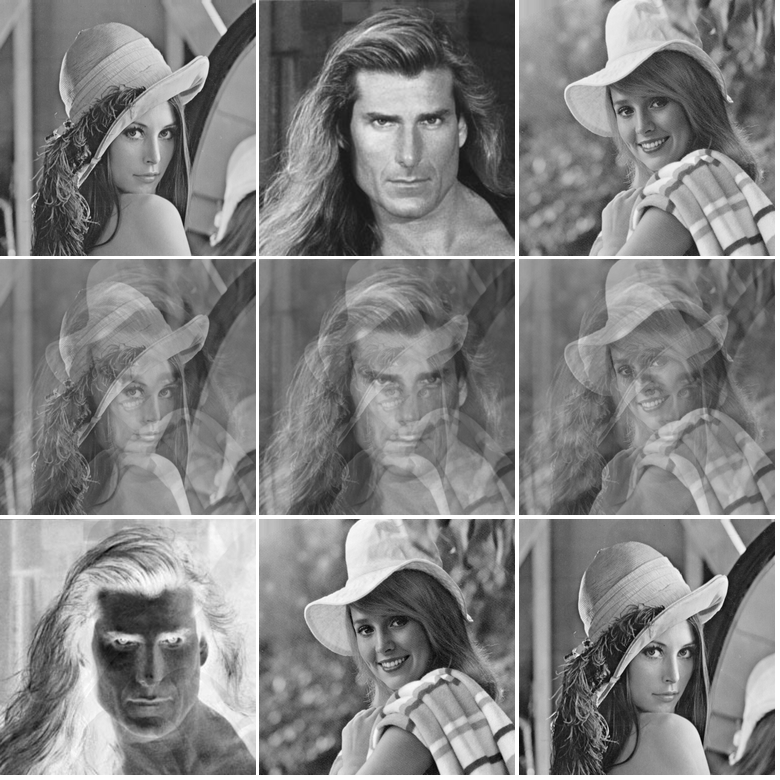
\includegraphics[width=0.5\textwidth]{img/imagemixing}}
						  \caption{$3$ images mixed linearly then unmixed}
						\end{figure}
					\end{myblock}\vfill
					\begin{myblock}{Independent images basis}
						This time the quantity of interest is $W$ the unmixing matrix, $s$ representing the random coefficients in the ICA basis of natural images. In this setting the columns of $A$ form the basis and the columns of $W$ the detectors.
						\begin{figure}[H]
							\centering
							\subfloat{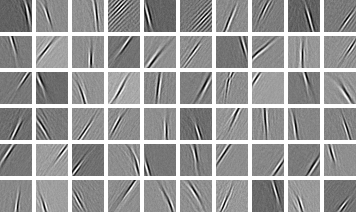
\includegraphics[width=0.5\textwidth]{img/basis}}
							\caption{ICA basis of the $3$ previous images}
						\end{figure}
					\end{myblock}\vfill
					\begin{myblock}{Conclusion}
						Treating the problem as a semi-parametric problem gives a tractable solution. The problem becomes a pure optimization problem and improvements can be achieved with better optimization techniques that exploits the geometry \cite{Shen2009}.
						\\
						ICA has proven to be invaluable to many real world problems such as EEGs processing and also can bring insights to many unsupervised learning problems such as compressend sensing of images.
					\end{myblock}\vfill
					\begin{myblock}{References}
						\footnotesize
						\bibliographystyle{abbrv}
						\bibliography{./Biblio}
					\end{myblock}\vfill
		}\end{minipage}\end{beamercolorbox}
	\end{column}
\end{columns}
\end{frame}
\end{document}
